\section{The Symbol-to-State Binding Gap}
\label{sec:gap}

\begin{table}[t]
  \centering
  \caption{\textbf{Matched interface comparison on Paired128.} Interface columns are call accuracies (\%). The final column is the source-image-balanced Physicalized-minus-Numeric effect in percentage points, so it need not equal the difference of rounded call accuracies.}
  \label{tab:main}
  \scriptsize
  \resizebox{\textwidth}{!}{% Generated by build_evidence_registry.py
\begin{tabular}{lrrrr}
\toprule
Model & Numeric & Calibrated & Physicalized & Balanced $\Delta_{P-N}$ \\
\midrule
Doubao Seed 2.1 Turbo & 66.94 & 63.71 & 75.54 & +8.40 \\
Gemini 3.6 Flash & 74.33 & 71.10 & 90.86 & +16.28 \\
Qwen3.8-Max & 73.52 & 74.06 & 90.05 & +16.08 \\
\midrule
Three-model majority & 75.54 & 73.79 & 91.13 & \textbf{+15.30} \\
\bottomrule
\end{tabular}
}
\end{table}

\subsection{Physicalized Candidates Improve Verification}

Table~\ref{tab:main} reports the complete paired result. Doubao, Gemini, and Qwen improve by source-image-balanced effects of $+8.40$, $+16.28$, and $+16.08$ points. Gains remain positive at every candidate distance. The three-model majority rises from \MajorityNumeric\% to \MajorityPhysicalized\%; its balanced effect is \MajorityBalancedGain{} points, 95\% CI $[\MajorityGainLow,\MajorityGainHigh]$. At the call level, Physicalized removes 63.7\% of the majority errors remaining under Numeric.

All-model correctness rises from \AllCorrectNumeric\% to \AllCorrectPhysicalized\%, with 147 majority repairs and 31 breaks. Figure~\ref{fig:ladder} shows the same trajectory for each model. Calibrated remains close to Numeric: 63.71, 71.10, and 74.06\% versus 66.94, 74.33, and 73.52\%. Correct branch, unit, direction, and tick value therefore do not supply the missing absolute correspondence between the candidates and the photographed scale.

\begin{figure}[t]
  \centering
  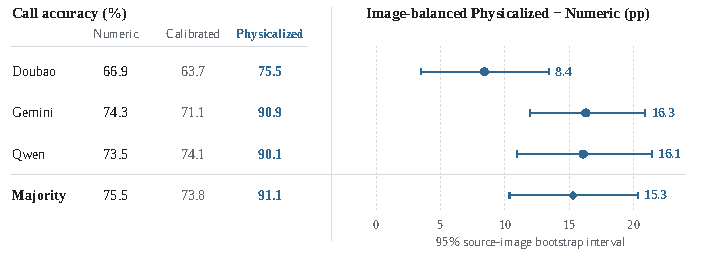
\includegraphics[width=\textwidth]{fig2_representation_ladder.pdf}
  \caption{\textbf{Matched interface comparison.} Left: call accuracy for the three interfaces. Right: source-image-balanced Physicalized-minus-Numeric effects with 95\% source-image bootstrap intervals. Calibration remains near Numeric, while physicalizing candidate states produces a consistent gain.}
  \label{fig:ladder}
\end{figure}

The result is not driven by one instrument type. Removing each major family leaves a $+12.06$ to $+18.19$-point majority effect, and every source-image bootstrap interval remains above zero. In particular, the gain is $+12.06$ points without rulers and $+18.19$ without thermometers, the largest family.

\subsection{Physicalization Gains Persist Across Reasoning Budgets}
\label{sec:reasoning}

Fresh45 provides matched effort matrices for additional model settings. Physicalized $-$ Numeric effects remain positive for Gemini at minimal/medium/high effort ($+16.30/+19.63/+18.15$ points), GPT-5.6 Terra at low/medium/high ($+16.30/+17.41/+14.81$), and Qwen at low/medium/extra-high ($+24.81/+25.56/+27.04$). GPT-5.6 Sol at medium effort independently rises from 81.85\% to 91.85\%. Low-effort Physicalized also exceeds high-effort Numeric by 10.00, 13.70, and 25.56 points for Gemini, Terra, and Qwen. Increasing language-side computation does not substitute for the missing image-specific state map.

\subsection{Complementary Probes of the Gap}

The automatic proposers expose target and lattice estimates before human geometry is used for evaluation. On held-out images, Doubao localizes the target within one tick on 62.60\% of 123 images but reconstructs the lattice within one tick on only 24.39\% (median errors 0.45 versus 3.40 ticks). Gemini reaches 46.77\% and 41.94\% over 124 images. Thus, a target can be found even when the numerical anchors are bound to the wrong local lattice. Figure~\ref{fig:mechanism} shows both this component asymmetry and the larger effect on two-endpoint measurements.

\begin{figure}[t]
  \centering
  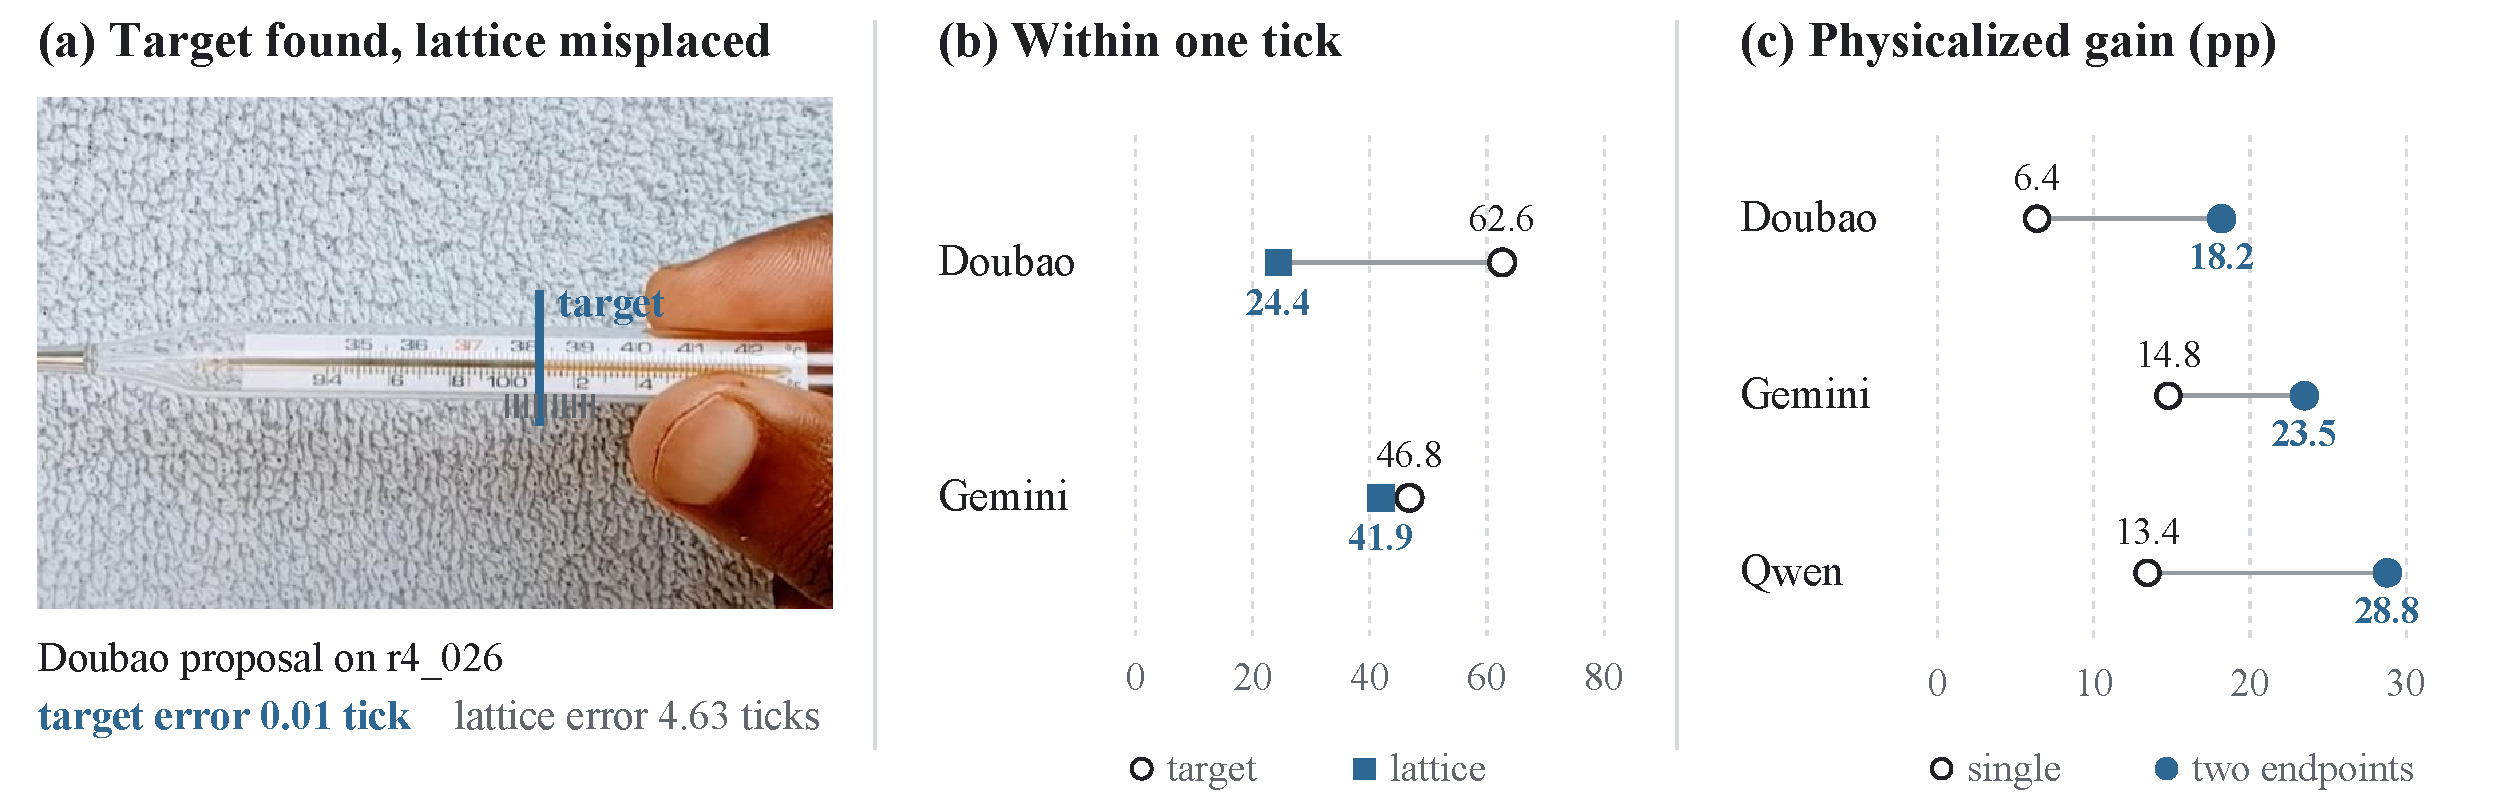
\includegraphics[width=\textwidth]{fig3_mechanism.pdf}
  \caption{\textbf{Complementary probes.} A real proposal can localize the measured boundary while placing the local lattice incorrectly. Aggregate target and lattice errors show the same separation, and Physicalized gains are larger for two-endpoint ruler spans than for single-state tasks. Source image: MeasureBench~\cite{lin2026measurebench}, CC BY-SA 4.0; cropped and annotated by the authors.}
  \label{fig:mechanism}
\end{figure}

\subsection{Two-Endpoint Ruler Spans Increase the Burden}

On 22 ruler-span images, Numeric accuracy ranges from 49.22\% to 57.81\% across Doubao, Gemini, and Qwen. Physicalization gains $+18.18$, $+23.48$, and $+28.79$ points, compared with $+6.37$, $+14.78$, and $+13.44$ on 106 single-state images. Explicitly instructing Doubao and Qwen to read both endpoints and subtract still leaves Physicalized ahead by $+19.70$ and $+35.61$ points. The result points to an upstream grounding bottleneck: two image states must first be aligned to the same scale.
